\section{Supplementary Material}
\label{ch2_supp}

\subsection{Numerical Methods}
\label{sec:Numerical}
We expand upon our description of the numerical methods used in our simulations. We consider varying system sizes from  $N=10^2$ to $N=10^{300}$ with time varying from $t=0$ to $t= 5000 \log(N)$. We simulate such large systems by utilizing the full range of quadruple-precision floating point numbers and making approximations to the binomial distribution when dealing with sizes beyond our precision limits. These approximations are necessary given the limitations of our precision and do not seem to affect the behavior of the system in any significant manner. In particular, for a site $x$ at time $t$ where the number of particles, $N(x,t)$, is below $2^{31}$ we use the C++ Boost integer implementation of a binomial distributed random number generator to choose the number of particles that will move right versus left. Above $2^{31}$ the integer implementation overflows and we instead  approximate the binomial distribution by a Gaussian distribution of mean $N(x,t) B(x,t)$ and variance $N(x,t)  B(x,t) (1 - B(x,t))$, as dictated by the central limit theorem. For sufficiently large $N(x,t)$, the variance itself will fall outside of the precision of a quadruple floating point number. This occurs when $N(x,t) > 10^{64}$, above which we approximate the binomial simply by its mean. The number of particles that move right is then $N(x,t) B(x,t)$. Psuodo-code of the simulation is given:

\begin{enumerate} 

 \item Start $N$ particles at $x=0$
 \item For each site:
  \subitem draw $B(x,t)$ from $\mathcal{U}_{[0, 1]}$
  \subitem if ($N(x, t) > 10^{64}$)
   \subsubitem $N(x+1, t+1) = N(x, t)B(x,t)$
   \subsubitem $N(x-1, t+1) = (1-B(x,t))N(x,t)$
  \subitem else if ($2^{31} < N(x, t) < 10^{64}$)
   \subsubitem $\mu = N(x,t)B(x,t)$
   \subsubitem $\sigma^2 = N(x,t)B(x,t)(1-B(x,t))$
   \subsubitem $N(x+1, t+1)$ is drawn from $\mathcal{N}(\mu, \sigma^2)$
   \subsubitem $N(x-1, t+1) = N(x, t) - N(x+1, t+1)$
  \subitem else if ($N(x, t) < 2^{31}$)
   \subsubitem $N(x+1, t+1)$ is drawn from $\mathrm{Bin}(N(x,t), B(x,t))$
   \subsubitem $N(x-1, t+1) = N(x,t) - N(x+1, t+1)$
\end{enumerate}

where $\mathcal{U}_{[0, 1]}$ is the random uniform distribution on the range $[0, 1]$, $\mathcal{N}(\mu, \sigma^2)$ is the Gaussian distribution with mean $\mu$ and variance $\sigma^2$, and $\mathrm{Bin}(n, p)$ is the Binomial distribution with number of trials $n$ and probability $p$. Note that our simulation differs from Monte Carlo, or agent based, simulations because we can group all the particles at a site together and iterate over each site. Our code is available at \url{https://github.com/CorwinLab/RWRE-Simulations}.

When estimating the statistics (e.g. mean and variance) for $\maxnt,\envnt$ and $\snt$, the optimal manner would be that for each $N$ and $t$ we simulate a large number of environments and then build up histograms for the behavior of these quantities with one data point corresponding to one environment. Of course, in numerically computing the quantities for time $t$, we naturally compute them for all times smaller than $t$ too, but for the same environment. Moreover, $\envnt$ can be computed simultaneously for all $N$ and $t$ relative to the same environment, providing even further computational savings. We employ this computationally efficient approach to couple together the estimation for different values of $N$ and $t$ to the same pool of environments. There is a cost, however, to doing this. For example, the statistics that we numerically compute for $\maxnt$ for time $t$ and time $t'$ will themselves be correlated since they are derived from studying the same collection of environments. This correlation seems to be short-lived in time though, and is only evident upon zooming into the numerical measurements, for instances as in the inset in Fig. \ref{fig:QuantileVar} of the main text.

\subsection{Asymptotic Theory Results}
\subsubsection{SSRW $\boldsymbol{\maxnt}$}\label{sec:SSRW}For the SSRW where $B(x,t)\equiv 1/2$, we use the same notation $p(x,t)$ and $P(x,t)$, dropping the $\mathbf{B}$ subscript. Now assume that the ratio $\hat{t} = t/\log(N)$ tends to some finite value. As explained in the main article, if $\hat{t}<(\log(2))^{-1}$ then $N\gg 2^t$. In that case, $p(t,t)=2^{-t} \gg 1/N$ which means that it is highly likely that there are many particles occupying the right-most site at $x=t$. This implies that $\mean{\maxnt}\approx t$ and $\var{\maxnt}\approx 0$.

When $\hat{t}> (\log(2))^{-1}$, the maximal random walk at time $t$ will likely occur significantly below $t$ and have non-trivial fluctuations which we now describe. For the SSRW, observe that $p(2k-t,t) =2^{-t} {t\choose k}$ for $k=0,\ldots, t$. Thus, using Stirling's formula for binomial coefficients (or more generally using Cramer's theorem from the large deviation theory for sums of independent identically distributed random variables) we arrive at the asymptotic for $v\in (0,1)$ that
\begin{equation}\label{eq:ldp}
P(vt,t) \approx e^{- t I_{\mathrm{SSRW}}(v)}\quad\textrm{where}\quad I_{\mathrm{SSRW}}(v) = \frac{1}{2}\big((1+v)\log(1+v) + (1-v)\log(1-v)\big).
\end{equation}
$I_{\mathrm{SSRW}}(v)$ is known of as the large deviation rate function for the SSRW.

We may now combine this with Eq. \eqref{eq:maxpb}  of the main text to show that
$\maxnt$ is approximately distributed as a Gumbel random variable with location
$\mu \approx t\hat v$ and shape  $\beta= 1/I_{\mathrm{SSRW}}^{\prime}(\hat v)$, where $\hat v=I_{\mathrm{SSRW}}^{-1}(1/\hat{t})$ (here $f^{-1}$ means the inverse function and not the reciprocal). A Gumbel random variable with location $\mu$ and shape $\beta$ has
\begin{equation}\label{eq:Gumbel}
\textrm{cumulative distribution function } e^{-e^{(-x-\mu)/\beta}},\quad \textrm{mean } \mu+\beta\gamma, \quad \textrm{and variance } \frac{\pi^2}{6}\beta^2,
\end{equation}
where $\gamma\sim .57721$ is the Euler-Mascheroni constant.


To see the above limit, observe that
\begin{align*}
&\mathrm{Prob}\big(\maxnt \leq t\hat{v}+x\big) = \big(1-P_{\mathbf{B}}(t\hat{v}+x,t)\big)^N \approx \big(1-  e^{- t I_{\mathrm{SSRW}}(\hat{v}+x/t)} \big)^N\\
&\approx \big(1-  e^{- t I_{\mathrm{SSRW}}(\hat{v}) - I'_{\mathrm{SSRW}}(\hat{v})x} \big)^N
=  \big(1-  N^{-1} e^{- I'_{\mathrm{SSRW}}(\hat{v})x} \big)^N \approx e^{-e^{- I'_{\mathrm{SSRW}}(\hat{v})x}}.
\end{align*}
The first equality follows from  Eq. \eqref{eq:maxpb}  of the main text, the second approximation uses \eqref{eq:ldp}, the third uses Taylor expansion, the fourth follows from the definition of $\hat v=I_{\mathrm{SSRW}}^{-1}(1/\hat{t})$, while the final one uses the approximation $(1-x/N)^{N}\approx e^{-x}$. Notice that in Taylor expanding we have assumed that lower order terms do not cause issues. This can be easily justified by going to further orders in the Stirling formula expansion.

Based on the above Gumbel asymptotics, we can now record the asymptotic form of the mean and variance of $\maxnt$ for the SSRW. Writing $\hat{v}(\hat{t})$ to make this dependence explicit and recalling that $\hat{t}= t/\log(N)$ we see that
\begin{equation}\label{eq:SSRWmeanvar}
\mean{\maxnt}\approx t\hat v\big(\tfrac{t}{\log(N)}\big) +  \frac{\gamma}{I_{\mathrm{SSRW}}^{\prime}\Big(\hat v\big(\frac{t}{\log(N)}\big)\Big)} ,\quad \var{\maxnt}\approx
 \frac{\pi^2}{ 6 \Big(I_{\mathrm{SSRW}}^{\prime}\Big(\hat v\big(\frac{t}{\log(N)}\big)\Big)\Big)^2}.
\end{equation}
Inverting $I_{\mathrm{SSRW}}$ to find $\hat v(\hat{t})$ is non-trivial though can be done numerically or in certain limits. For instance, noting that for $v$ near zero, $I_{\mathrm{SSRW}}\approx v^2/2$  we see that for $\hat{t}$ near infinity,  $\hat{v}(\hat{t})\approx \sqrt{2/\hat{t}}$ and hence
$I_{\mathrm{SSRW}}^{\prime}\big(\hat v(\hat{t})\big)\approx \sqrt{2/\hat{t}}$. From this and \eqref{eq:SSRWmeanvar} it follows that for $\hat{t}\gg  (\log(2))^{-1}$, asymptotically
$$
\mean{\maxnt}\approx \Big(\sqrt{2 \log(N)} + \frac{\gamma}{\sqrt{2 \log(N)}}\Big) t^{1/2},\qquad
\var{\maxnt}\approx \frac{\pi^2}{12}\frac{t}{\log(N)}.
$$
On the other hand, \eqref{eq:SSRWmeanvar} also shows that as $\hat{t}$ tends to $ (\log(2))^{-1}$ from above, the mean goes to $t$ and the variance goes to zero.

\subsubsection{RWRE $\envnt$}\label{sec:RWREenv}
Assume that the ratio $\hat{t} = t/\log(N)$ tends to some finite value exceeding $1$. The key theoretic result we use  here is due to \cite{barraquand_random-walk_2017}. They show that for $v\in (0,1)$,
%%
\begin{equation}\label{eq:bc}
\log\big(P_{\mathbf{B}}(vt,t)\big) = - t I(v)  + t^{1/3} \sigma(v)\chi_{t}\quad \textrm{where}\quad I(v) = 1- \sqrt{1- v^2},\quad\sigma(v) = \left(\frac{2 I(v)^2}{1-I(v)}\right)^{1/3}.
\end{equation}
Here $I(v)$ is the large deviation rate function and $\sigma(v) t^{1/3}$ is the scalings of the random environment-dependent fluctuations $\chi_t$ around that rate function. \cite{barraquand_random-walk_2017} showed that as $t\to\infty$, the distribution of $\chi_t$ converges to a Tracy-Widom GUE distribution $\chi$. For reference below, let us note that \cite{prahofer_universal_2000}
$$
\mu_\chi := \mean{\chi} \approx -1.771,\qquad \sigma_{\chi}^2 := \var{\chi}\approx .813.
$$

As in the case of the SSRW, we now solve for $\hat v=\hat v(\hat t)$ such that $P_{\mathbf{B}}(\hat vt,t)= 1/N$. Note that $\hat vt$ will then equal the $1/N$-quantile $\envnt$. From \eqref{eq:bc}, $\hat v$ must satisfy
\begin{equation}\label{eq:tIhat}
t I(\hat v) - t^{1/3} \sigma(\hat v) \chi_t =\log(N) = t/\hat{t}.
\end{equation}
Canceling $t$ and dropping the $t^{1/3}$ term momentarily yields to first order that $\hat v$ is given by
$$\hat v_0 = I^{-1}(1/\hat{t}) = \sqrt{1-(1-1/\hat{t})^2}.$$
We can now Taylor expand $I(\hat{v})$ and $\sigma(\hat v)$ in \eqref{eq:tIhat} around $\hat{v}=\hat{v}_0$ and solve for $\hat{v}$ to the next order. Doing so we find that
$$\hat{v} = \hat{v}_0 + t^{-2/3} \frac{\sigma(\hat{v}_0)}{I'(\hat{v}_0)} \chi_t + O(t^{-4/3}).$$
Recalling that $\hat{v} t$ is supposed to yield the $1/N$-quantile, we conclude that
\begin{equation}\label{eq:envntform}
\envnt = \hat v_0 t + t^{1/3} \frac{\sigma(\hat v_0)}{I'(\hat v_0)}  \chi_t + O(t^{-1/3}).
\end{equation}
From this we can extract the asymptotic mean and variance of $\envnt$. Written explicitly (i.e., plugging in $I$ and $\hat{v}_0$
) this yields the following asymptotic formulas
\begin{align*}
\mean{\envnt} &\approx M_1(N,t):= \Big(1-\big(1-\tfrac{\log(N)}{t}\big)^2\Big)^{1/2} t  +(\log(N))^{2/3} t^{-1/3}  \frac{2^{1/3} \big(1-\frac{\log(N)}{t}\big)^{2/3}}{\sqrt{1-\big(1-\frac{\log(N)}{t}\big)^2}} \mu_{\chi} \\
\var{\envnt}  &\approx V_1(N,t):= \Big(\frac{(\log(N))^{4/3}}{t^{2/3}}\Big)\frac{2^{2/3}\big(1-\frac{\log(N)}{t}\big)^{4/3}}{1- \big(1- \frac{\log (N)}{t}\big)^2} \sigma_{\chi}^2 ,
\end{align*}
where above we have used that
$$
\frac{\sigma(\hat{v}_0)}{I'(\hat{v}_0)}  = \frac{2^{1/3} \hat{t}^{-2/3} (1-1/\hat{t})^{2/3}}{\sqrt{1-(1-1/\hat{t})^2}}.
$$
For $\hat{t}=t/\log(N)$ large, it follows from the above expressions that
\begin{equation}\label{eq:varenvlogN}
\var{\envnt}  \approx  \sigma_{\chi}^2 \big(\tfrac{\log(N)}{2}\big)^{\frac{1}{3}} t^{\frac{1}{3}}.
\end{equation}
It is important to understand the order of the limits here. First we should fix $\hat{t}=t/\log(N)$ and take $N$ and $t$ to infinity. Then we take $\hat{t}$ large and find the above $1/3$ power-law. That said, with some additional work using the methods of  \cite{barraquand_random-walk_2017} it is possible to show that for the entire range $1\ll t/\log(N) \ll \log(N)$, this $1/3$ power-law persists. We will not provide the details for that here. However, below we will consider when $t$ is of order $(\log(N))^2$. In that case, for small $t$ in that range, we will find a perfect fit to the $1/3$ power-law, thus agreeing with the assertion that this power-law persists over the full range $1\ll t/\log(N) \ll \log(N)$.

\medskip
Now assume that the ratio $\hathat{t} = t/\log (N)^2$ remains strictly positive and finite as $N$ and $t$ tend to infinity.
While \cite{barraquand_random-walk_2017} probes $P_{\mathbf{B}}(x,t)$ for $x$ linearly growing with $t$, \cite{barraquand_moderate_2020} probes the regime where $x$ grows like $t^{3/4}$. They show that for $v\in (0,\infty)$,
\begin{equation}\label{eq:BLD}
\log\big(P_{\mathbf{B}}(v t^{3/4},t)\big)\approx  -\frac{v^2 t^{1/2}}{2} - \frac{\log(t)}{4} + \log(v) - \frac{v^4}{12}+ h(0,v^4)
\end{equation}
where $h(y,s)$ denotes the (random) height at spatial position $y$ and time $s$ of the {\it narrow wedge solution to the Kardar-Parisi-Zhang (KPZ) equation}
$$\partial_s h(y,s) = \tfrac{1}{2}\partial_y^2 h(y,s) + \tfrac{1}{2} \big(\partial_y h(y,s)\big)^2 +  \xi(y,s)$$
driven by space-time white noise $\xi$, see \cite{kardar_dynamic_1986, corwin_kardar_2012}. Using this result, we will be able to prove this other $(\log(N))^2$ time scale.

We may solve  \eqref{eq:BLD} perturbatively (as in the $\log(N)$ case) for $\hathat{v}$ such that $P_{\mathbf{B}}(\hathat{v}t^{3/4},t)= 1/N$. The $1/N$-quantile $\envnt=\hathat{v}t^{3/4}$ is then given by
$$
\envnt \approx \hathat{v}_0 t^{3/4} + \frac{t^{1/4}}{\hathat{v}_0}\left(h(0,\hathat{v}^4) - \frac{\hathat{v}_0^4}{12} -\log(\hathat{v}_0)\right) + O(t^{-1/4})\quad\textrm{where}\quad \hathat{v}_0 = 2^{1/2}\hathat{t}^{-1/4}.
$$
From this we can explicitly compute the asymptotics of the mean and variance as
\begin{align}\label{eq:var_longtime}
\nonumber \mean{\envnt} &\approx M_2(N,t):=  \big(2 t\log(N)\big)^{1/2} +\sqrt{\tfrac{t}{2\log(N)}}\mean{h\Big(0,\tfrac{4 (\log(N))^2}{t}\Big)}\\
\var{\envnt} &\approx V_2(N,t):= \tfrac{t}{2\log(N)} \cdot \var{h\Big(0,\tfrac{4 (\log(N))^2}{t}\Big)}.
\end{align}
Notice that in the mean we have dropped the lower order contributions from the terms $\frac{\hathat{v}_0^4}{12}$ and $\log(\hathat{v}_0)$.
The values of $\mean{h(0,s)}$ and $\var{h(0,s)}$ for varying $s>0$ can be computed numerically through evaluation of the Fredholm determinant formula from \cite{sasamoto_one-dimensional_2010,calabrese_free-energy_2010,dotsenko_bethe_2010,amir_probability_2011}.
The result of this computation is recorded as Fig. 3 of \cite{prolhac_height_2011}. In particular, the horizontal axis (labeled $t$ in  \cite{prolhac_height_2011}) corresponds to our $s$ variable, and the red circles record the value of $\mean{\frac{h(0,s)+\frac{s}{24}}{(s/2)^{1/3}}}$ while the blue triangles record the values of $\var{\frac{h(0,s)+\frac{s}{24}}{(s/2)^{1/3}}}$ (note that the $s/24$ shift here does not change the variance as it is deterministic). For $s>.33$ we approximate the mean and variances by interpolating between the numerically evaluated values in \cite{prolhac_height_2011} (S. Prolhac kindly provided the data set used to create Fig. 3 in that paper). For $s<.33$ we use the short-time behavior of the KPZ equation explained below for our values of the mean and variance.

There are two key asymptotics for $h(0,s)$ derived in \cite{sasamoto_one-dimensional_2010,calabrese_free-energy_2010,dotsenko_bethe_2010,amir_probability_2011}:
$\frac{h(0,s)+\frac{s}{24}}{(s/2)^{1/3}}\approx \chi$ as $s\to\infty$ where $\chi$ is a Tracy-Widom GUE distributed, and
$h(0,s)\approx -\tfrac{1}{2}\log(2\pi s) +s^{1/4} \pi^{1/4}2^{-1/2} G$ as $s\to 0$ where $G$ is standard Gaussian distributed.
These imply corresponding asymptotics for the mean and variance. In particular, as $\hathat{t}\to 0$,
$$
\var{\envnt} \approx \sigma_{\chi}^2 2^{-1/3} \log(N) \hathat{t}^{1/3}  = \sigma_{\chi}^2 \big(\tfrac{\log(N)}{2}\big)^{\frac{1}{3}} t^{\frac{1}{3}}
$$
which agrees perfectly  with \eqref{eq:varenvlogN}. This shows that the long-time behavior in the $t=O(\log(N))$ scaling regime and the short time behavior in the $t=O(\log (N)^2)$ scaling regime match even up to the pre-factor. This strongly suggests the $1/3$ power-law in Eq. \ref{I-eq:varqnt} of the main text for the entire regime $1 \ll t/\log(N) \ll \log (N)$.

On the other hand, from the short-time KPZ asymptotic we find that as $\hathat{t}\to \infty$,
$$
\var{\envnt} \approx \frac{1}{2} \pi^{1/2} t^{1/2}
$$
thereby recovering Eq. \eqref{eq:varqnt} for the regime $t\gg (\log(N))^2$ in the main text. This indicates that for finite $N$ and $t$ it is necessary to stitch together the two regimes to get a reasonable formula for $\var{\envnt}$.
We have found that an error function centered at $t=(\log(N))^{3/2}$ with a width of $(\log(N))^{4/3}$ produces a smooth transition between the two regimes. Thus, our final expression for the asymptotic mean and variance is given by
\begin{equation}
\label{eq:Var-Total}
\varasy{\envnt} = \frac{1-\text{erf}\left(\tfrac{t-(\log(N))^{3/2}}{(\log(N))^{4/3}}\right)}{2} V_1(N,t)+ \frac{1+\text{erf}\left(\tfrac{t-(\log(N))^{3/2}}{(\log(N))^{4/3}}\right)}{2}V_2(N,t),
\end{equation}
provided that $t\geq \log(N)$ and $0$ for $t<\log(N)$. Here $\text{erf}(x)= 2/\sqrt{\pi} \int_{0}^{x} e^{-t^2}dt$ is the error function. This construction is shown in Fig. \ref{fig:Interpolation}.
On the other hand, such stitching is unnecessary when it comes to the mean since the large $t$ behavior of $M_1(N,t)$ matches the behavior of $M_2(N,t)$ all the way as $t\to \infty$. This can be seen through direct asymptotics of the formulas and is illustrated in Fig. \ref{fig:MeanInterpolation}. On this account, we simply take
\begin{equation}
\label{eq:Mean-Total}
\meanasy{\envnt} =M_1(N,t).
\end{equation}

\begin{figure}[h]
\begin{center}
 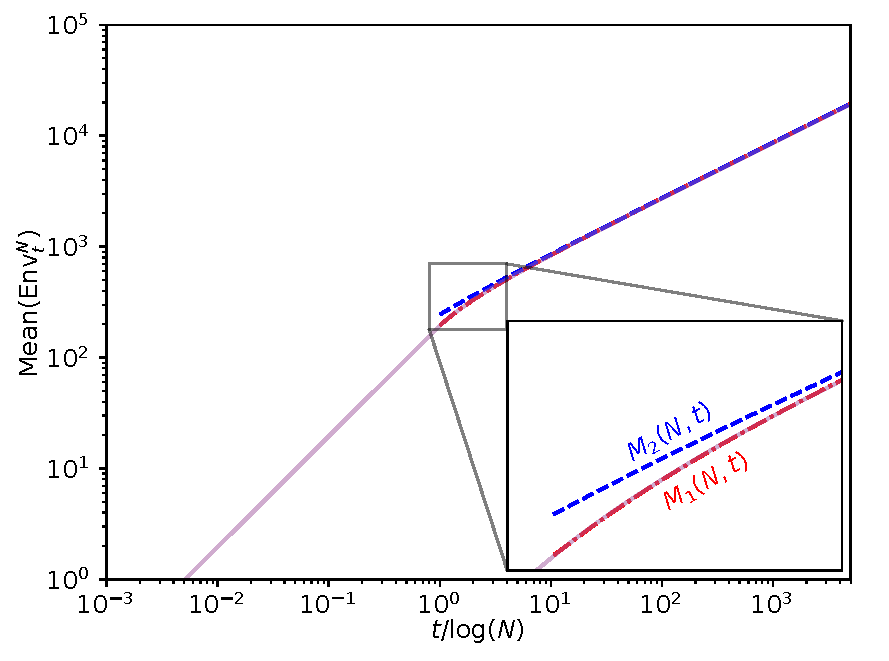
\includegraphics[width=0.8\columnwidth]{ch2_supplement/MeanInterpolation.pdf}
 \caption{The asymptotic mean functions $M_1(N,t)$ and $M_2(N,t)$ are plotted for $N=10^{85}$ in red and blue dashed lines, respectively. They agree closely for the full range of $t>\log(N)$ and also match the numerically measured values $\meannum{\maxnt}$ given by the purple curve (which is linear, as expected, until roughly time $t=\log(N)$).}
 \label{fig:MeanInterpolation}
\end{center}
\end{figure}

\begin{figure}[h]
\begin{center}
 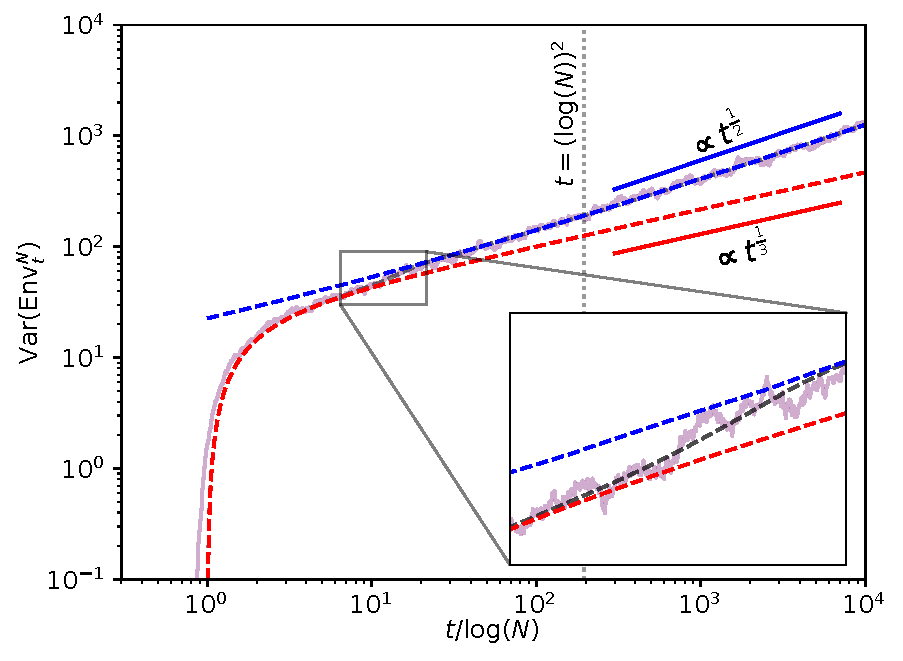
\includegraphics[width=0.8\columnwidth]{ch2_supplement/Interpolation.pdf}
 \caption{The asymptotic variance functions $V_1(N,t)$ and $V_2(N,t)$ are plotted for $N=10^{85}$ in red and blue dashed lines, and the stitched together formula for $\varasy{\envnt}$ from \eqref{eq:Var-Total} is plotted as the black dashed line. The purple curve is the numerically measured curve  $\varnum{\envnt}$. The inset shows how the stitching captures the transition between the two asymptotic curves $V_1$ and $V_2$, and the solid lines show the asymptotic power-laws that $V_1$ and $V_2$ demonstrate as $t\to\infty$. The vertical dotted line indicates the regime crossover at $t=(\log(N))^2$.}
 \label{fig:Interpolation}
\end{center}
\end{figure}

\subsubsection{RWRE $\snt$ and $\maxnt$}\label{sec:RWRE_Sam}
Assume for the moment that $t= \hat{t}\log(N)$ for $\hat{t}>1$. Then \eqref{eq:bc} implies that
$$
P_{\mathbf{B}}( \envnt + x,t) =\exp\Big(-tI\big(\tfrac{\envnt}{t} +\tfrac{x}{t}\big) + t^{1/3}\sigma\big(\tfrac{\envnt}{t} +\tfrac{x}{t}\big)\chi_t\Big)\qquad \textrm{and} \quad P_{\mathbf{B}}( \envnt,t) = \frac{1}{N}.
$$
If we Taylor expand to the next order in the exponential we find
\begin{align*}
P_{\mathbf{B}}( \envnt + x,t)&\approx \exp\Big(-tI\big(\tfrac{\envnt}{t}\big)-I'\big(\tfrac{\envnt}{t}\big)x + t^{1/3}\sigma\big(\tfrac{\envnt}{t}\big)\chi_t\Big)\\
&=\frac{1}{N} e^{-I'\big(\tfrac{\envnt}{t}\big)x} \approx\frac{1}{N}  e^{-I'(\hat{v}(\hat{t}))x}.
\end{align*}
The Taylor expansion requires a bit of explanation. We expand $I\big(\tfrac{\envnt}{t} +\tfrac{x}{t}\big) \approx I\big(\tfrac{\envnt}{t}\big) + I'\big(\tfrac{\envnt}{t}\big) \tfrac{x}{t}$ to first order. The similar expansion of $\sigma$ would produce a lower order term. However, there is a subtlety that we should point out. The $\chi_t$ random variable implicitly depends on $x$ as well. Namely, if we look at the random transition probability as we vary around $\envnt$, the fluctuations of this quantity will vary with $x$. However, we assume here that this fluctuation does not contribute to leading order. This assumption would be true if, for instance, $\chi_t$ looked locally like a random walk with independent and identically distributed intervals. This property is believed to be universal to models in the KPZ class and thus it is reasonable to assume that the same holds here. We do not attempt to justify this theoretically beyond this heuristic, though note that it yields very good agreement with our numerical simulations. The final approximation in the above string of equations involves replacing $I'\big(\tfrac{\envnt}{t}\big)x$ by $I'(\hat{v}(\hat{t}))x$ which relies on the fact that $\tfrac{\envnt}{t}\approx \hat{v}_0$ to highest order.

Combining the above deduction with \eqref{maxpb} in the main text and  $(1-x)^N\approx e^{-xN}$ (for $x$ small) yields
\begin{equation}\label{eq:SNT}
\mathrm{Prob}(\maxnt\leq \envnt + x) \approx \Big(1-\frac{1}{N}  e^{-I'(\hat{v}(\hat{t}))x}\Big)^{N}
\approx e^{-e^{-I'(\hat{v}(\hat{t}))x}}.
\end{equation}
If we define $\snt$ by the equality $\maxnt=\envnt+\snt$ then the above calculation shows that $\snt$ is asymptotically independent of $\envnt$ and asymptotically is Gumbel distributed with location and shape parameters
$$\mu(t)=0,\qquad \beta(t)=1/I'(\hat{v}(\hat{t})) = (\hat{t}-1)(2\hat{t}-1)^{-1/2}\approx (\hat t/2)^{1/2}$$
where the approximation is for $\hat{t}\gg 1$. This justifies the addition law for variances (Eq. \eqref{I-eq:varadd} in the main text)
\begin{equation}\label{eq:addlaw}
\var{\maxnt}\approx \var{\envnt}+\var{\snt}
\end{equation}
and (using the Gumbel variance formula in \eqref{eq:Gumbel}) this also justifies Eq. \eqref{I-eq:varnst} of the main text which provides the asymptotic formula for the variance (we also record that the asymptotic mean is 0)
\begin{equation}\label{eq:sntmeanvar}
\meanasy{\snt} =0,\qquad \varasy{\snt} = \frac{\pi^2}{6} \frac{\big(\frac{t}{\log(N)} -1\big)^2}{2\frac{t}{\log(N)} -1}\approx \frac{\pi^2}{12} \frac{t}{\log(N)},
\end{equation}
where the approximation is for $\hat{t}\gg 1$.

Putting together  \eqref{eq:Var-Total}, \eqref{eq:Mean-Total}, \eqref{eq:addlaw} and \eqref{eq:sntmeanvar} we conclude that
\begin{align}
\begin{split}
\label{eq:Var-Totalmaxnt}
\meanasy{\maxnt} &= M_1(N,t),\\
\varasy{\maxnt} &= \frac{1-\text{erf}\left(\tfrac{t-(\log(N))^{3/2}}{(\log(N))^{4/3}}\right)}{2} V_1(N,t)+ \frac{1+\text{erf}\left(\tfrac{t-(\log(N))^{3/2}}{(\log(N))^{4/3}}\right)}{2}V_2(N,t)\\&\quad+ \frac{\pi^2}{6} \frac{\big(\frac{t}{\log(N)} -1\big)^2}{2\frac{t}{\log(N)} -1}.
\end{split}
\end{align}

The above calculation assumed $\hat{t}=t/ \log(N)$ converges to a finite value. However, in a similar manner based on \eqref{eq:BLD} we can probe the behavior when $\hathat{t}= t/(\log(N))^2$ converges to a finite value. This behavior agrees perfectly with the large $\hat{t}$ limiting behavior above. Thus, we conclude that the formula for $\varasy{\snt}$ should hold for all $t\gg \log(N)$.

Fig. \ref{fig:MaxMean} show our asymptotic theory formulas for the mean of the maximal particle fit closely with our numerical simulations.


\begin{figure}[ht]
\begin{center}
 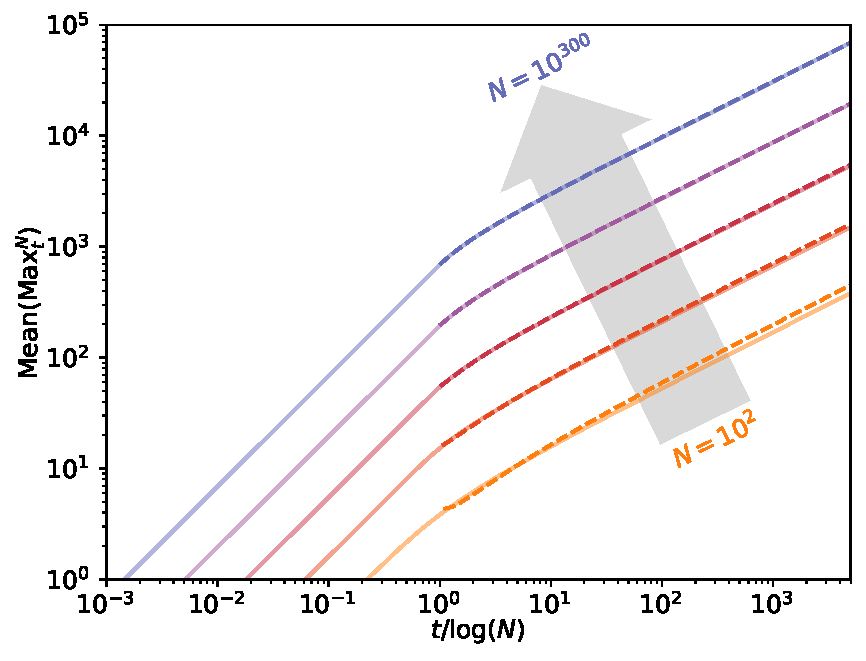
\includegraphics[width=0.8\columnwidth]{ch2_supplement/MaxMean.pdf}
 \caption{The mean position of the maximal particle location (solid line) for $N=10^2, 10^{7}, 10^{24}, 10^{85}$ and $10^{300}$ for $10000$, $5000$, $1000$, $500$ and $500$ instantiations of the environment, respectively. The theoretical prediction (dashed line) given in Eq. \eqref{eq:Var-Totalmaxnt} is also shown. We find the theoretical predictions for the mean position of the maximum particle, $\mean \maxnt$, are in agreement with the data.}
 \label{fig:MaxMean}
\end{center}
\end{figure}
